\documentclass{article}
\usepackage{graphicx}
\usepackage[utf8]{inputenc} % allow utf-8 input
\usepackage[T1]{fontenc}    % use 8-bit T1 fonts
\usepackage{hyperref}       % hyperlinks
\usepackage{url}            % simple URL typesetting
\usepackage{booktabs}       % professional-quality tables
\usepackage{amsfonts}       % blackboard math symbols
\usepackage{nicefrac}       % compact symbols for 1/2, etc.
\usepackage{microtype}      % microtypography
\usepackage{xcolor}         % colors
\usepackage{amsmath}
\begin{document}

\title{15-618 Final Project Report\\ Parallel TSP Solvers}

\author{
    Yujun Qin (yujunq), Dongxiao Han (dongxiah)\\
    Carnegie Mellon University\\
    Pittsburgh, PA 15213 
}

\maketitle
\begin{abstract}
The Traveling Salesman Problem (TSP) is a famous NP-hard problem featuring high computational complexity to compute an exact solution. In this report, we demonstrate the parallel implementations using multi-core CPUs and GPUs to accelerate the solving of TSP for both exact and heuristic solutions. We will show that a 64-core CPU can have close-to-linear speedup and a GPU can achieve up to 5,000x speedup compared with a single-core CPU solution.
\end{abstract}

\section{Background}
\subsection{Travelling Salesman Problem}
    The Traveling Salesman Problem (TSP) is a famous NP-hard problem. It asks for the shortest route to visit all the cities in the list exactly once. The TSP problem has applications in various fields for planning optimization. Since the TSP problem is NP-hard, finding exact solutions to this problem is very time consuming. Therefore, we expect that parallelism can be exploited to accelerate the process of solving the TSP problem. In the scope of our project, we will solve the symmetric TSP problem using Euclidean distances in a 2D Cartesian coordinate. Define $N$ as the number of cities, and $d_{ij}$ is the distance between node $i$ and $j$.
\subsection{Held-Karp Algorithm}
    An exact solution to the TSP problem is the Held–Karp algorithm, which is a dynamic programming solution of time complexity O($N^22^N$) \cite{hk}. Let $f(i, V)$ represents the shortest route starting from node $i$, visiting all the nodes in set $V$ exactly once, and return to the root point $s$. Let $d_{ij}$ be the distance from node $i$ to $j$. The transfer function can be written as:
    $$f(i, V) = 
    \begin{cases}
        \min(d_{ij} + f(j, V - \{j\})) \text{ for } j \text{ in } V & V \neq \emptyset \\
        d_{is} & V = \emptyset
    \end{cases}$$
    The target we will compute is $f(s, V - \{s\})$, which represents the shortest tour length beginning from $s$, visiting all the other nodes exactly once, and returning to $s$.
\subsection{Ant Colony System (ACS) Algorithm}
    The ant colony system algorithm is a distributed algorithm that is applied to the TSP\cite{acs}. In the ACS, a set of cooperating agents called ants cooperate to find good solutions to the TSP problem. Ants indirectly communicate using a pheromone they deposit on the edges of the graph when moving on the edges. The ACS is inspired by the natural behavior of ants and the ACS performs well in the quality of result when combined with local optimizations like 2-opt or 3-opt.\\
    
    The high level idea of ACS is to let ant with shortest tour deposit pheromone inversely proportional to the total length of the whole tour. Ants randomly choose the next hop with the probability proportional to the pheromone on the edge. In this way, ants will consolidate the pheromone on short tours. Beyond that, ACS allows the ants to choose the best edge with certain probability (called exploitation), and after choosing an edge, ants will immediately update the pheromone on the edge to encourage exploration for other ants. 
\section{Approach}
\subsection{Held-Karp Algorithm: CUDA}
\subsubsection{Overview}
    In order for CUDA to efficiently execute the Held-Karp algorithm, states should be computed in a bottom-up way. We arrange the computation in the following way:
    \begin{enumerate}
        \item Calculate all the sets with the same number of nodes in a batch, and batches are in the order from empty set to full set. (i.e. Calculate $f(i, V)$ for all $|V| = 0$, then $|V| = 1$, ... until $|V| = N - 1$ assuming $N$ is the number of all nodes.)
        \item In each batch, calculation is launched as a CUDA kernel. Each thread ID is mapped to a unique pair of $(i, V)$ in this stage.
        \item Each thread searches the previous states, calculates the minimum, and update the state of itself.
    \end{enumerate}
    We will fix the root point to be node 0 in this section. Therefore, 0 will not appear in $i$ or $V$ and the following indexing will be 1-based. (e.g. First bit means the least significant bit.)
\subsubsection{State Compression}
   In order to efficiently store the computed values, we need to create a mapping from a integer of thread ID to a unique pair of $(i, V)$. Considering the complexity of the TSP problem and the algorithm, it can only handle a small number of nodes. Therefore, it is possible to encode the set $V$ to a 64-bit integer, where the $k$-th bit represents the presence of node $k$ in the set, and we call this number the \textit{expanded state}.\\
    
    Based on the above definition, for the pair $(i, V)$, the expanded state of $V$ always has 0 on the $i$-th bit, and therefore, we can skip the $i$-th bit and shift all the left bits to the right, and we get the \textit{compressed state}. In this way, given an positive integer $i$ and another non-negative integer $v < 2^{N-1}$, we can easily map the pair $(i, v)$ to the pair $(i, V)$ required by the algorithm.\\
    
    For example, for an input with 5 cities $0, 1, 2, 3, 4$,
    $$(1, \{2, 3\}) \xrightarrow{Expanded State} (1, 0b0110) \xrightarrow{Compress} (1, 0b011) = (1, 3)$$
    $$(3, \{4\}) \xrightarrow{Expanded State} (3, 0b1000) \xrightarrow{Compress} (3, 0b100) = (3, 4)$$
    $$(2, \emptyset) \xrightarrow{Expanded State} (2, 0b0000) \xrightarrow{Compress} (2, 0b000) = (2, 0)$$\\
    
    The state compression provides an efficient way to represent state indexing in a 2D array $f[N-1][2^{N-1}]$. We will use this array in its expanded 1D form to store the computed values.
\subsubsection{Thread Indexing}
    The state compression itself is not enough for effective computation in CUDA. In stage $k$, we need to compute for all the states where there are exactly $k$ ones in their binary compressed state (i.e. $|V| = k$). We should be able to map any integer from 0 to the total number of such sets, to a unique set that satisfies the requirement.\\
    
    A simple way is to find the $(i+1)$-th smallest state that satisfies the requirement for the integer $i$. In order to find the number efficiently, we need to first find how many such numbers exists. There are ${n\choose k}$ integers with $n$ bits, of which $k$ are ones. We will use the above conclusion to get the $i$-th number with $k$ ones. We first reduce our target to finding the leftmost one, and we find it in the following way:\\
    
    Assume the leftmost is on the bit with index $p$ (i.e. the $(p+1)$-th bit). Then the order of this number $q$ must lie in the range $$\sum_{j=k}^{p}{j\choose k} < q \leq \sum_{j=k}^{p+1}{j\choose k}$$Therefore, we can iterate until the sum is accumulated to larger than $i$ and then $p$ is the leftmost set bit. \\
    
    After the leftmost bit is fixed, we can subtract the last sum before exceeding $i$ from $i$, and decrement $k$ by 1, and we can continue the process recursively until all bits are set. (Recursions are converted to iterative methods considering limited depth of recursion on CUDA.)\\
    
    Using the technique above, we are now able to assign a unique pair of $(i, V)$ with $|V| = k$ to each thread using the thread ID.

\subsection{ACS Algorithm: CUDA}
\subsubsection{Overview}
    To exploit the parallelism behind the ACS algorithm, there are two directions. The first is the trivial parallelism between ants. Ants does not communicate directly. They are just sharing the pheromone map. However, the ACS algorithm does not require enough ants to fill all the threads, we also need to have parallelism for the execution of one ant. Therefore, we assign an ant to a whole CUDA block, and the ant will exploit the parallelism in the block to accelerate calculation. Using this method, we can use in-block shared memory for communication within the block and also have the parallelism between ants.
\subsubsection{In-block Parallelism}
    We first identify the most time consuming part that can be parallelized. When an ant is deciding on which node should be the next hop, it is required to find all the nodes that have not been visited. Then 
    \begin{enumerate}
        \item The node with the most pheromone should be found if this will be an exploitation.
        \item All the possible next hops should be picked randomly with the probability proportional to the pheromone on the edge if we need exploration.
    \end{enumerate}
    In order to efficiently parallelize the above operations, we used the in-block reduction and scan from CUB\cite{cub}. Finding the maximum is trivial using the reduction. We will focus on how to efficiently select a random node.
\subsubsection{Parallel Node Selection}
    Before moving to the actual process, we could simplify the question to: With an array of floats $p$ ($p_i\geq 0$ for all $i$) and the same number of threads as the array size, how can we choose a node with the probability proportional to the value? The intuitive solution would be:
    \begin{enumerate}
        \item Inclusive scan the array to get the prefix sum in the shared array $s$.
        \item Generate a random float $r$ in the range of 0 to $s_{N-1}$ (the sum of all floats).
        \item Each thread check if $r$ falls in the range $s_{i-1}$ and $s_i$. If yes, write to the shared result variable.
    \end{enumerate}
    However, we are processing more nodes than the threads we have (512 threads in a block in our implementation). We address this issue with a two-level design:
    \begin{enumerate}
        \item All the node indices with the same remainder divided by the block size are assigned to the same group.
        \item We have exact the same number of groups and threads.
        \item The group has the value equal to the sum of its members.
        \item We first select a group using the method above, and then within the group, we do the same to select the actual node.
    \end{enumerate}
    Using the above two-level design, we are able to handle $2^{18} = 262144$ number of nodes, which is enough for this project.
\subsubsection{Local Updates}
    All the ants are required to do the local update to the pheromone after selecting the next hop. The pheromone should be updated with $\tau = (1-\rho)\tau + \Delta\tau$. We decide not to synchronize the reading, which adds the risk of reading stale data. However, we are optimistic that such conflicts rarely happens, and the consequence of read stale data is negligible. This operation also cannot be done atomically by default. We implemented the \texttt{atomicAxpy} function using the \texttt{atomicCAS} to do the above action atomically to avoid race conditions in writing. 
\subsubsection{Parallel 2-opt}
    2-opt is a simple optimization which finds all pairs of edges that can be re-routed to improve the overall tour length, until no further changes can be made. Performing 2-opt requires multiple iterations over all pairs of edges, and performing 2-opt swap requires reversing a lot of nodes. To efficiently perform 2-opt, we first launch a kernel which assigns a thread to each pair of edges to check if an improvement can be made. If so, we launch another kernel to perform one change and repeat. 
    
\subsection{Held-Karp Algorithm: OpenMP}
\subsubsection{Overview}
    To avoid unnecessary barriers and critical sections, a combination of candidate cities are created before running in parallel.\\
    The process of initialization:
    \begin{enumerate}
        \item Create an unordered map called $combinations$ where key represents the number of candidate cities and the value represents multiple lists. Each list is a combination of $k$ cities from $K-1$ cities, where $K$ is the total number of cities.
        \item Initialize a $graph$ using unordered map with 3 levels of keys, where level 1 is the target city id, level 2 is the number of cities that will go across from the initial city, level 3 is a string that combines specific city ids that will go across.
    \end{enumerate}
    The process of parallelism:
    \begin{enumerate}
        \item For different combinations from 1 to all the cities, the number of subsets in each combination is large enough and they don't have dependent relationship that can run in parallel with significant speedup.
    \end{enumerate}
\subsubsection{Structures of data containers}
    Using cities = [1, 2, 3, 4, 5] and 2 CPU cores as an example. Assume the departure city is always city 1.\\\\
    $combinations$:
        $$combinations[1] = [[2], [3], [4], [5]]$$
        $$combinations[2] = [[2, 3], [2, 4], [2, 5], [3, 4], [3, 5], [4, 5]]$$
        $$combinations[3] = [[2, 3, 4], [2, 3, 5], [2, 4, 5], [3, 4, 5]]$$
    Suppose it is running the 3rd loop, i.e. $combinations[3]$, the working tasks will be assigned in this way: CPU1 will run [2, 3, 4] and [2, 3, 5], CPU2 will run [2, 4, 5] and [3, 4, 5]. When the number of total cities increases, the number of tasks will also increase significantly. For example, a combination of 10 cities from 20 cities is 184,756. When applying these tasks to each core, the effect of parallelism is significant.\\\\
    $graph$:
        $$graph[3][2]['2,4'] = min(graph[2][1]['2'] + dist[2][3], graph[2][1]['4'] + dist[4][3])$$
    Suppose the current loop will start from city 1, go across 2 cities, and the target city is city 3. Within one core, it will check the minimum distance and store the distance to the graph.
    

\subsection{ACS Algorithm: OpenMP}
\subsubsection{Overview}
    ACS algorithm can be generally split into three parts in one iteration: find the current best path for all ants, update pheromones locally and update pheromones along the shortest path.\\
    The process of initialization:
    \begin{enumerate}
        \item Initialize a vector $ant_path$ that stores the path for each ant. Ants will start at
        different cities.
        \item Create a map $graph$ that stores pheromones from one city to another city.
    \end{enumerate}
    The process of parallelism:
    \begin{enumerate}
        \item Ants run in different cores to find its current best path. Once found, pheromones will be updated for the path. Since it is possible that at least two ants go across the same city, $critical$ is used here to let only one core can update $graph$.
        \item Once found the shortest path, updating pheromones along the path using different cores.
    \end{enumerate}
\subsubsection{Structures of data containers}
    Using 3 ants, 5 cities, 2 CPU cores as an example.\\\\
    $ant\_path$:
        $$ant\_path[0] = [1, 2, 3, 4, 5, 1]$$
        $$ant\_path[1] = [2, 1, 3, 4, 5, 2]$$
        $$ant\_path[2] = [3, 1, 2, 4, 5, 2]$$
    Each array in $ant\_path$ represents an ant and its path. The slot in the array will be updated via swapping with the following slots.\\\\
    $graph$:
        $$graph[city_i][city_j] = pheromone_k$$
    Ants will select path based on pheromones on each edge. Although $graph$ is shared across multiple cores, the update can happen simultaneously when the edges that need update are different.


\subsection{Held-Karp Algorithm: MPI}
\subsubsection{Overview}
    Similar to the implementation of OpenMP, the version of MPI also uses $combinations$ and $graph$. Since $combinations$ is a static data container, we should assign jobs for each core based on the the number of subsets in $combinations$. But for $graph$, since an updated distance for one state depends on some distances calculated from a previous state, the distances must be communicate across all the nodes.\\
    The process of parallelism:
    \begin{enumerate}
        \item Each core will create $combinations$ with the same contents. Jobs will be created for each core to assign some subsets that they will run later to update $graph$.
        \item Each core will run the subsets and only update graph within the subsets.
        \item Gather the updated information within the graph for each core to core 1 and then broadcast all of them to each core. Then, each core updates its graph with the information that are calculated by other cores.
    \end{enumerate}

\subsubsection{Communication}
    Jobs are assigned according to the number of subsets for combination in $combinations$. Within each core, graph is only updated with the cities in the assigned subsets. Thus, the local update should be gathered, broadcast, and updated again. Since the structure of $graph$ is a multi-layer map, 3 keys and 1 value are stored as 4 vectors.

\subsection{ACS Algorithm: MPI}
\subsubsection{Overview}
    Except using $ant\_dist$ and $graph$ as mentioned in the version of OpenMP, jobs are assigned for each core. In each job, it contains several ants that will be executed by different cores.\\
    The process of parallelism:
    \begin{enumerate}
        \item Once the current best path is found all the ants, the path will be updated are gathered, broadcast and each core will update the same edge simultaneously.
        \item During the process of identifying the best path from the start city to the end city, the total distance of ants will keep adding. Once finishing exploration, there is no need to gather and broadcast the whole path to calculate distance again.
        \item Once the global best path is found in each core, the $graph$ will be updated to add more pheromones on the global best path.
    \end{enumerate}
\subsubsection{Communication}
    Jobs are assigned based on the number of ants. When setting a small number of ants, some cores will be idle, which is not helpful to have significant speedup. It means that the number of ants must be larger than the number of CPU cores.

\section{Results}

The implementation of ACS Algorithm via CUDA, OpenMP, MPI uses the same default values of hyper-parameters. $\beta$ (=2.0) is the distance coefficient that is used to calculate the weighted pheromone when selecting the next city across the path. $\tau$ (=0.9) is the probability of using ACS state transition rule; otherwise, use the traditional state transition rule. $\rho$ (=0.1) is the weight to update local pheromones. $\alpha$ (=0.1) is the weight to update global pheromones.




\subsection{Speedup: OpenMP vs MPI}
\subsubsection{Held-Karp Algorithm}
    A limitation of our implementation is that the combinations of subsets are initialized before running in parallel. The number of cities limits the number of combinations that CPU can calculate. When the number of cities is over 20, the running time of initialization is quite long. The program will be killed due to memory issue when the number of cities is over 25. Thus, we only use 20 cities as the largest problem size.\\\\
    Figure~\ref{fig:exact_openmp_mpi} shows that the speedup across different cores and cities. For OpenMP, when the number of cities is 10 running on more cores, the increase of speedup is significantly lower than 15 cities and 20 cities. Two reasons can explain this trend. Firstly, the number of tasks that run in each core can benefit the speedup of OpenMP. The number of combinations for 10 cities starts at ${10\choose1}$, and then ${10\choose2}$, which is smaller than the number of cores in some loops. The utilization of cores is low. Some cores will be idle when the size of combinations increase at first and decrease at last. Another reason is false sharing. Although the number of assigned tasks is small when using more cores, the cache size assigned to each core decreases. The workload for each subset is always fixed, which means that one core always runs k times for load of distances whatever the number of subsets that are assigned. Thus, false sharing will happen when loading the distance in $graph$ from memory and then causing miss when the local cache is full. However, when looking at the speedup of 15 cities and 20 cities when running on 64 cores, it looks like the above explanation is contradictory. The speedup of 20 cities keep increasing, rather than decreasing. When comparing the difference of them, the increase of the number of combinations for 20 cities is super fast than 15 cities. The largest number of subsets for 20 cities is 184,756 (i.e. ${20\choose10}$), which is 733 times larger than 252 (i.e. ${10\choose5}$). It means that OpenMP can provide significant speedup when the assigned tasks in each core is large. Thus, if the problem size is large (20 cities is exponentially larger than 10 cities), the positive effect of the number of tasks exceeds the negative effect of false sharing.\\\\
    For MPI, the speedup is quite lower than OpenMP. The biggest reason is that the cost of communication is very high. The feature of communication in the implementation is that the frequency of communication is low but the scale of communication is large. The number of data that needs to be gathered to update $graph$ is fixed whatever how many subsets are assigned to each core. Since the update of $graph$ for the next loop needs all of updated distance for the previous loop, the updated distance that is executed by different cores must be broadcast to all cores for each loop. When the size of subsets increases, the cost of communication also increases. As a result, if each core must calculate data that is based on a large amount of global previous states and the states must be consistent across all the cores, the cost of message passing must be very high. In that situation, using MPI is not a sensible choice.\\\\

    \begin{figure}
        \centering
        \centerline{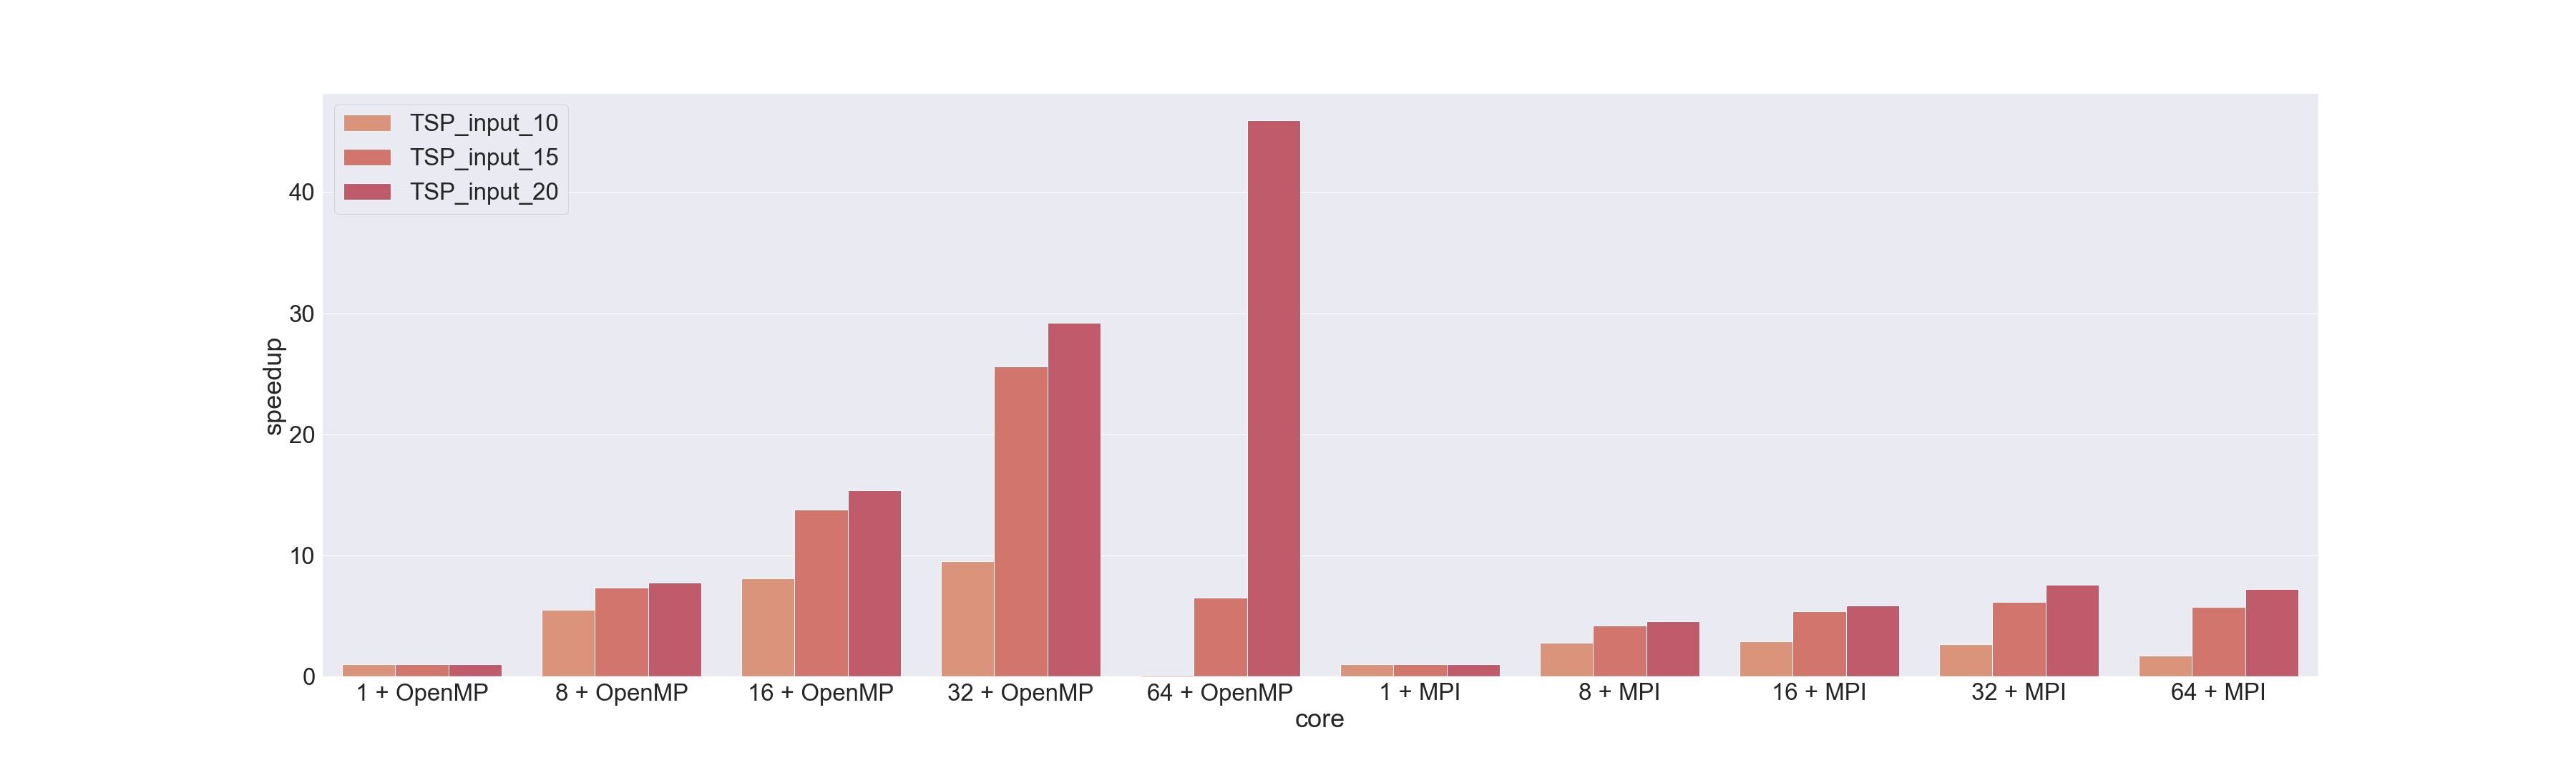
\includegraphics[scale=0.17]{exact_openmp_mpi.png}}
        \caption{Speedup across 1|8|16|32|64 cores with different number of cities using Held-Karp Algorithm}
        \label{fig:exact_openmp_mpi}
    \end{figure}


\subsubsection{ACS Algorithm}
    Figure~\ref{fig:acs_openmp_mpi} shows the speedup using higher scale with different number of cores. Except the fixed hyper-parameters mentioned at the very beginning of this section, the number of ants set in this experiment equals to 60\% of the number of cities. The reason of setting dynamic ratio is that it can balance an increasing workload when the scale of the problem increases. As you can see, when the number of cores is 64, the difference of speedup is closed among different scales when comparing the same settings of exact algorithm, which is contributed by the longer running time for each task. All the cores are running, no one is idle. One conclusion we can get when comparing the implementation of Held-Karp and ACS is that OpenMP can achieve significant speedup when the number of assigned tasks in each core is large and each task should have the closed running time.\\\\
    For MPI, the speedup is better than the one of Held-Karp. The feature of communication is that the frequency of communication is high but the scale of communication is small. Thus, to have a significant speedup when using MPI, programmers must avoid gathering and broadcasting too many data to every core.\\\\
    When comparing OpenMP and MPI, both achieves acceptable speedup when the number of cores increases. The whole trend of speedup for OpenMP is better than MPI. One key factor that could cause the low speed for OpenMP is barrier and critical section. If our implementation of OpenMP does not initialize data containers in advance, the effect of speedup will be terrible. As for MPI, the reason of low speedup is caused by two actions: gather and broadcast. Although ants can find their path in each core, the granularity of the update of pheromones on the graph must be shared by all ants for each loop. Thus, the update must be gathered from each core and then broadcast all the updates to all cores, which is time-consuming. If one problem doesn't need update the state based on a global one, MPI can achieve a better speedup.
    
    \begin{figure}
        \centering
        \centerline{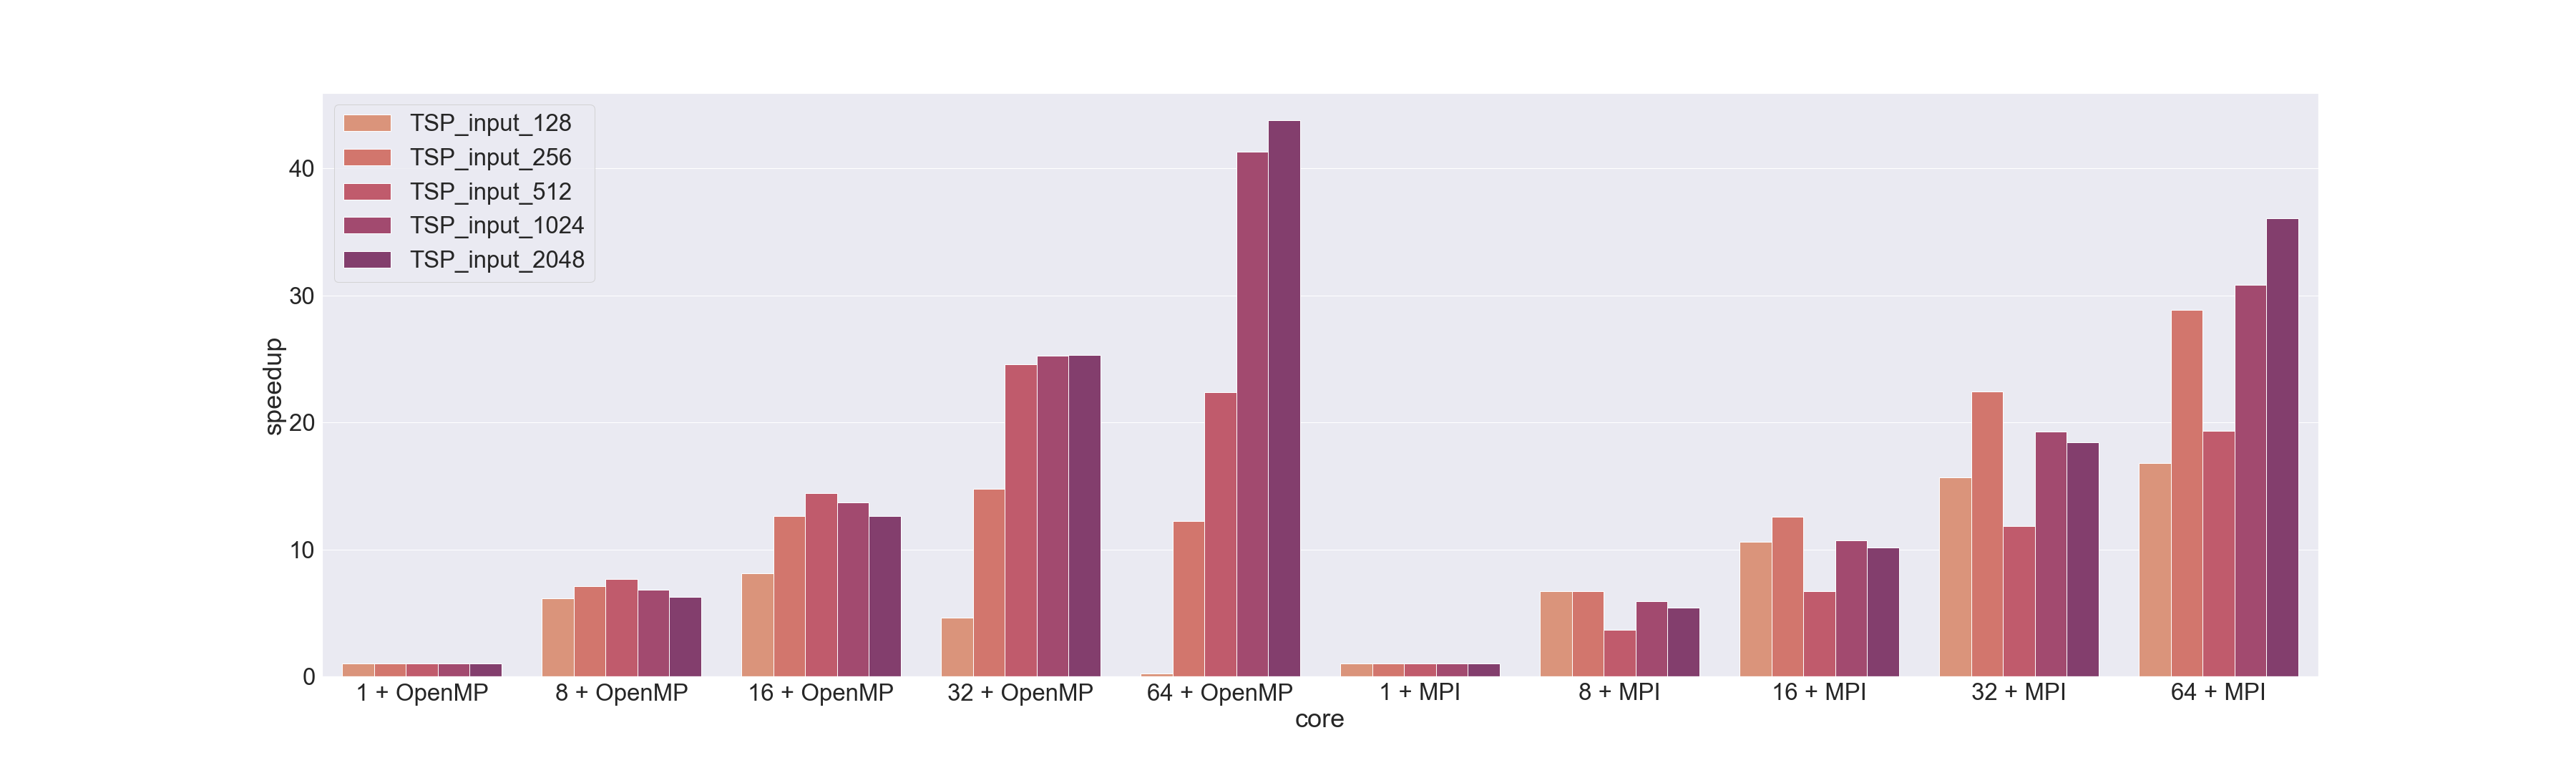
\includegraphics[scale=0.17]{acs_openmp_mpi.png}}
        \caption{Speedup across 1|8|16|32|64 cores with different number of cities using ACS Algorithm}
        \label{fig:acs_openmp_mpi}
    \end{figure}



\subsection{CUDA}

\subsubsection{Comparison with CPU}
We use an NVIDIA RTX 2080 graphics card to test the performance. Although they are tested on different architectures and different implementations, we are presenting the results to show the huge performance improvement using a GPU. The number of ants used in both algorithms are synchronized. The results are presented in Table~\ref{tab:cpu_gpu}. Approximately over 100x performance speedup is observed compared with a 64-core CPU, and 5000x speedup compared to a single-core CPU. 
\begin{table}[]
    \centering
    \begin{tabular}{c|c|c|c}
        Algorithm & CPU (1 thread) & CPU (64 threads) & GPU \\\hline
        Held-Karp (20 nodes) & 107s & 2.3s & 0.0057s  \\ \hline
        ACS (2048 nodes, 1 iteration) & 578s & 13.2s & 0.105s \\
    \end{tabular}
    \caption{The performance of running TSP algorithms on different processors. The CPU is  AMD EPYC 7742. The GPU is NVIDIA RTX 2080.}
    \label{tab:cpu_gpu}
\end{table}
\subsubsection{Held-Karp Algorithm}
We measured the execution time for the Held-Karp with the problem size. The result is shown in Figure~\ref{fig:hk_size}. We observed that the time grows exponentially as expected. We also present the shortest route is drawn for an input with 27 nodes in Figure~\ref{fig:hk_27}.
\begin{figure}
    \centering
    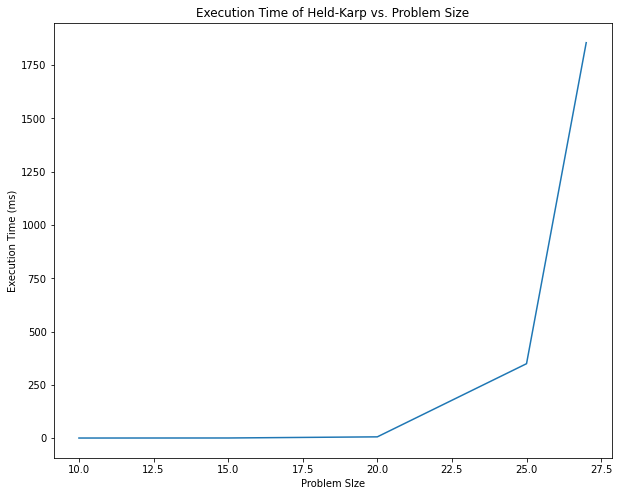
\includegraphics[width=0.8\textwidth]{hk_size.png}
    \caption{Execution Time of Held-Karp vs. Problem Size}
    \label{fig:hk_size}
\end{figure}
\begin{figure}
    \centering
    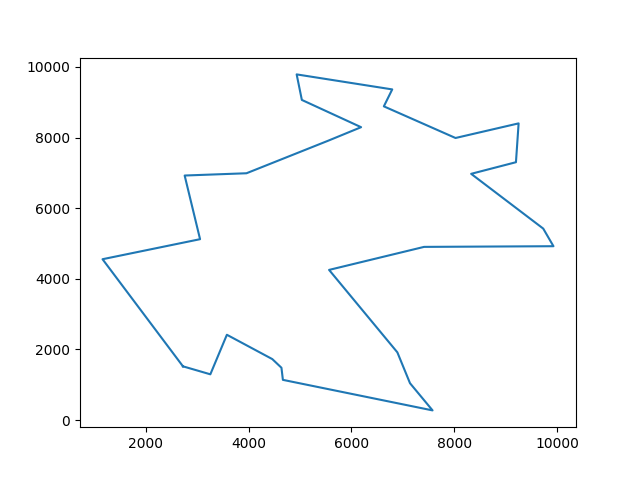
\includegraphics[width=0.8\textwidth]{hk_27.png}
    \caption{The output tour for an input with 27 nodes.}
    \label{fig:hk_27}
\end{figure}

\subsubsection{Number of Ants for ACS Algorithm}
With the huge speedup using the GPU, we are now able to analyze the hyper-parameters. We gather the results over the 2048 nodes input. As shown in the Figure~\ref{fig:ant_conv}, the speed of convergence grows slightly with more ants. However, as ant number is over 128, the execution time grows dramatically, which does not justify the extra convergence speed. Therefore we think 128 is a good number of balance between convergence speed and execution time. 
\begin{figure}
    \centering
    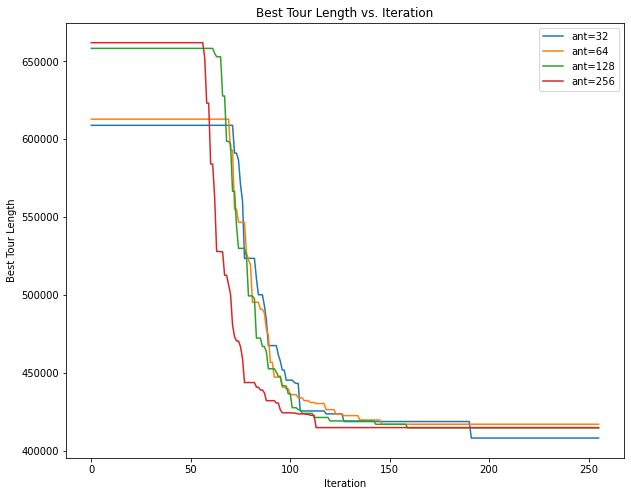
\includegraphics[width=0.8\textwidth]{ant_convergence.png}
    \caption{Best Tour Length vs. Iteration}
    \label{fig:ant_conv}
\end{figure}

\begin{figure}
    \centering
    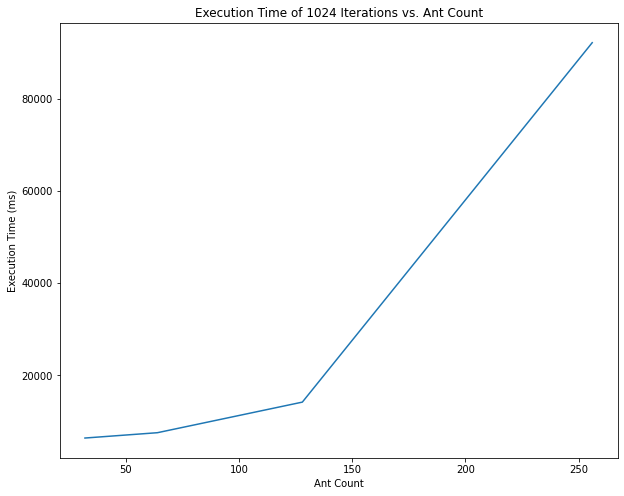
\includegraphics[width=0.8\textwidth]{ant_time.png}
    \caption{Execution Time of 1024 Iterations vs. Ant Count}
    \label{fig:ant_time}
\end{figure}


\subsubsection{ACS Execution Time}
Using 128 ants and 256 iterations, we have the relationship of execution time with the problem size. The result is presented in Figure~\ref{fig:acs_size}. The curve is close to a quadratic function, which is expected as the ACS has the time complexity O($N^2$).

\begin{figure}
    \centering
    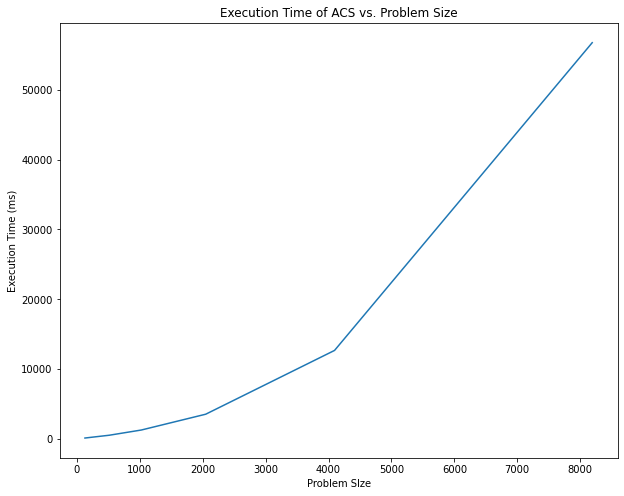
\includegraphics[width=0.8\textwidth]{acs_size.png}
    \caption{Execution Time of ACS vs. Problem Size}
    \label{fig:acs_size}
\end{figure}


\subsubsection{Using 2-opt for ACS Algorithm}
We tested three different 2-opt strategies:
\begin{enumerate}
    \item No 2-opt: No 2-opt operations are performed.
    \item Last 2-opt: Perform one 2-opt operation at the end of the last iteration.
    \item Every 2-opt: Perform 2-opt operation in every iteration.
\end{enumerate}
The results are shown in Figure~\ref{fig:2opt_conv}, Figure~\ref{fig:2opt_time} and Figure~\ref{fig:2opt_result}. We can see that 2-opt is very effective at reducing the total length, and the Last 2-opt strategy achieves the balance between execution time and route length. However, our 2-opt algorithm can still be improved (due to the time) by identifying all the pairs of edges that can be improved, and then conducting all the swaps before the next round of checking. We are currently running a naive solution which invokes a lot of additional kernel launches for 2-opt check,, which hurts the performance of Every 2-opt.
\begin{figure}
    \centering
    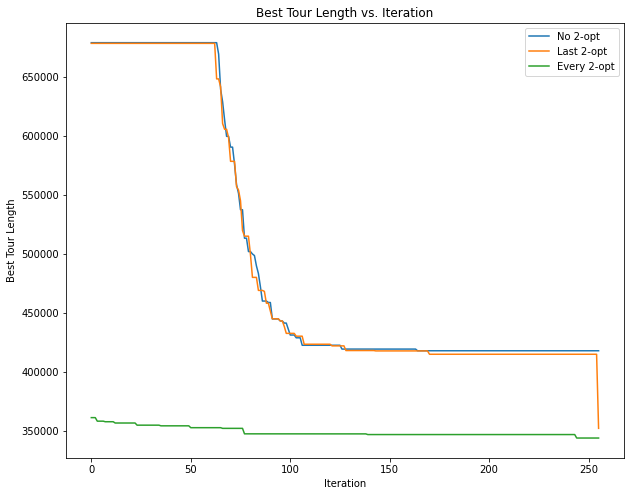
\includegraphics[width=0.8\textwidth]{2opt_conv.png}
    \caption{Best Tour Length vs. Iteration for Different 2-opt Strategies}
    \label{fig:2opt_conv}
\end{figure}
\begin{figure}
    \centering
    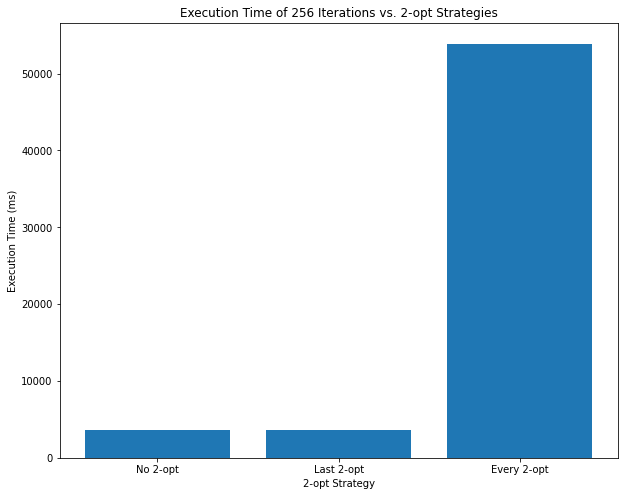
\includegraphics[width=0.8\textwidth]{2opt_time.png}
    \caption{Execution Time of 256 Iterations vs. 2-opt Strategies}
    \label{fig:2opt_time}
\end{figure}
\begin{figure}
    \centering
    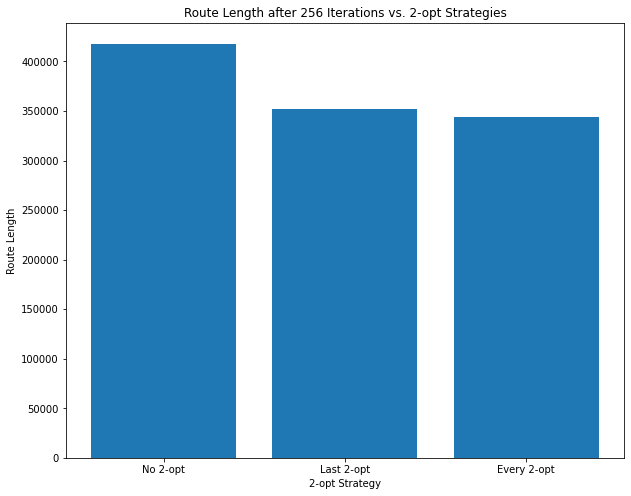
\includegraphics[width=0.8\textwidth]{2opt_result.png}
    \caption{Route Length after 256 Iterations vs. 2-opt Strategies}
    \label{fig:2opt_result}
\end{figure}

\subsubsection{Result Image}
    Figure~\ref{fig:8192} is the visualization of the output for ACS after 256 iterations using the Last 2-opt strategy.

\begin{figure}
    \centering
    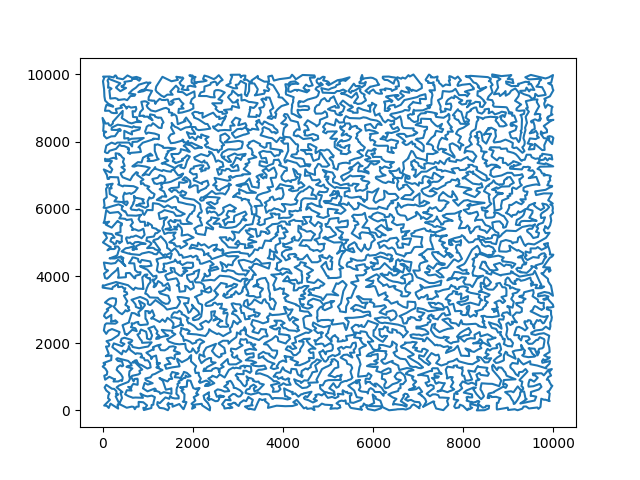
\includegraphics[width=0.8\textwidth]{8192.png}
    \caption{Output from ACS for the input with size 8192.}
    \label{fig:8192}
\end{figure}

\subsubsection{Limitations}
    The current GPU implementations can only handle 27 nodes for the Held-Karp algorithm and 8192 nodes for the ACS algorithm. The Held-Karp algorithm is limited by the global GPU memory, and the ACS algorithm is limited by the shared memory in a single block. The performance before we hit the cap is very satisfying, which is over 100x faster than our 64-core CPU performance. The performance is limited by communications and synchronizations within the block (e.g. waiting for thread 0 to generate a random number). We do not have explicit evidence to support this the statement, but we know the flaw when we are programming for this part. There are many \texttt{\_\_syncthreads()} in-block barriers used for the communication through the shared variables and synchronizations. The poor performance in the parallel 2-opt is known because the excessive launch of the check kernel does repeated jobs many times and wastes time. We know the way to improve the performance is by saving the edges that can be swapped in an array using exclusive scan and conduct all the swaps before the next check, but we don't have time for the implementation and debugging. Therefore we left the faster 2-opt optimization as a future direction of works.

\section{Distribution of Credits}
Our distribution of work is presented in Table~\ref{tab:credit}. We have a balanced distribution of work and the credit should be 50\%-50\%.
\begin{table}[!ht]
    \centering
    \begin{tabular}{c|c}
        Yujun Qin (yujunq) & Dongxiao Han (dongxiah) \\\hline
        Held-Karp: CUDA & Held-Karp: OpenMP \& MPI  \\ \hline
        ACS: CUDA & ACS: OpenMP \& MPI \\
    \end{tabular}
    \caption{Distribution of Work}
    \label{tab:credit}
\end{table}

%----------------------------------------------------------------------------------------
%	REFERENCE LIST
%----------------------------------------------------------------------------------------
%
% The following two commands are all you need in the
% initial runs of your .tex file to
% produce the bibliography for the citations in your paper.
\bibliographystyle{unsrt}
\bibliography{ref}  % sample.bib is the name of the Bibliography in this case

\appendix

\section{Appendix}


\end{document}